\documentclass{article}[12pt]
\usepackage{graphicx}

\title{[BSS]-Lab1-śr16-KrzysztofRudnicki}
\author{Krzysztof Rudnicki}
\begin{document} 
\maketitle 
\section{Generacja kluczy}
\paragraph{Wybrane liczby}
Wybrałem najniższe liczby pierwsze z przedziału 30 - 100 \\ 
p - 31, q - 37
\paragraph{Sprawdziłem że liczby 31 i 37 \textbf{są} pierwsze \\}
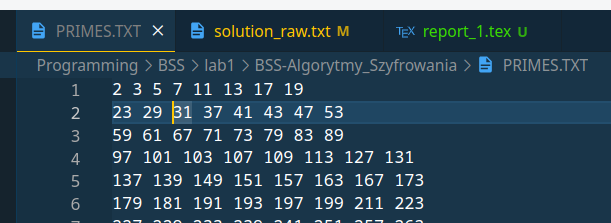
\includegraphics[width=1\textwidth]{one.png}
\paragraph{n = p * q = 31 * 37 = 1147}
\paragraph{$\rho(n) = (p-1) * (q-1) = 30 * 36 = 1080$}
\paragraph{Wybrałem liczbę e = 29}
Sprawdziłem, że jest względnie pierwsza względem 1080 \\ 
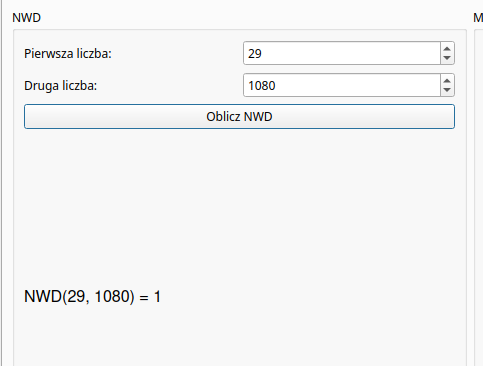
\includegraphics[width=1\textwidth]{two.png}
\paragraph{Liczba d = 149 \\}  
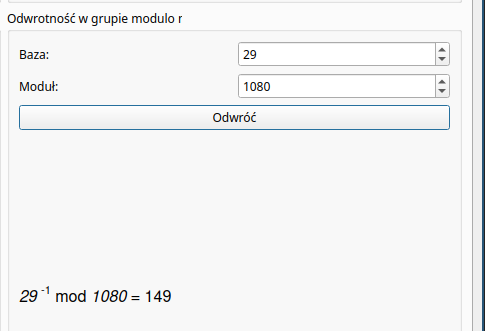
\includegraphics[width=1\textwidth]{three.png}
\paragraph{Klucz publiczny:  e = 29, n = 1147 \\ Klucz prywatny: d = 149, n = 1147}

\section{Szyfrowanie}
\paragraph{Fraza: DYZIO, litera: C}
\paragraph{Zakodowana Fraza: 68, 89, 90, 73, 79 \\ Zakodowana litera: 67}
\paragraph{Przygotowana wiadomość: PTAKI LATAJA KLUCZEM}
\paragraph{Wiadomość zaszyfrowana kluczem sesyjnym: KPWEB FWPWCW EFQDVZG \\}
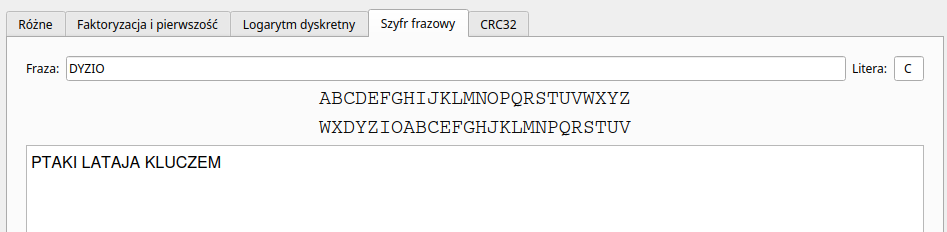
\includegraphics[width=1\textwidth]{four.png}
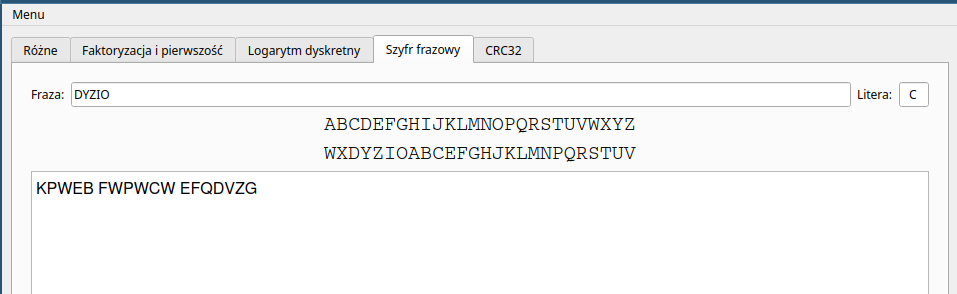
\includegraphics[width=1\textwidth]{five.png}
\paragraph{Klucz pobrany od kolegi:  $e_2 = 11, n_2 = 1763$}
\paragraph{Zaszyfrowany klucz sesyjny \\ Fraza: 168, 1621, 1632, 665, 178 \\ Litera: 1734 \\}
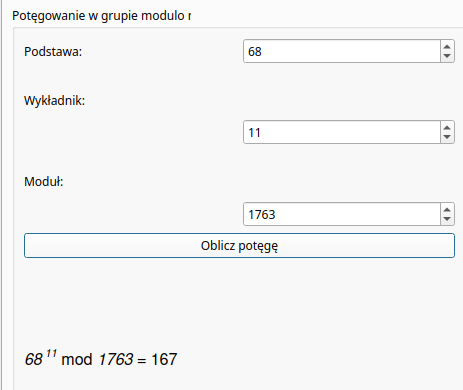
\includegraphics[width=1\textwidth]{six.png}
\paragraph{Klucz sesyjny przed zakodowaniem: DYZIO, C \\ Po Zakodowaniu: 68, 89, 90, 73, 79, \_67\_ \\ Po Zaszyfrowaniu: 168, 1621, 1632, 665, 178, \_1734\_}
\paragraph{Wiadomość przed zaszyfrowaniem: PTAKI LATAJA KLUCZEM \\ Wiadomość po zaszyfrowaniu: KPWEB FWPWCW EFQDVZG}

\section{Odszyfrowanie}
\paragraph{Otrzymałem klucz sesyjny:  423 65 693 1100 8 \_1073\_}
\paragraph{Odszyfrowałem go korzystając z mojego klucza prywatnego Klucz prywatny: d = 149, n = 1147}
\paragraph{Odszyfrowany klucz sesyjny: 107, 114, 48, 122, 97, \_111\_ \\}
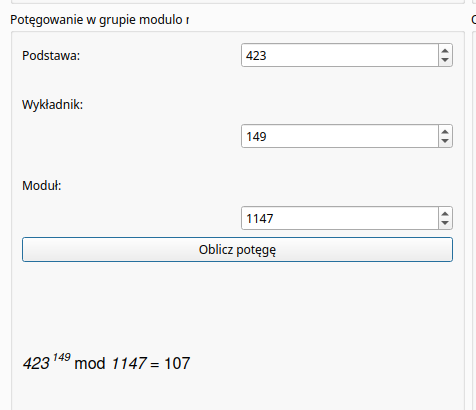
\includegraphics[width=1\textwidth]{seven.png}
\paragraph{Odszyfrowany klucz sesyjny odkodowałem: kryza, o}
\paragraph{Otrzymałem wiadomość: QNVVK XSLN BK WNNB GKC \\ } 
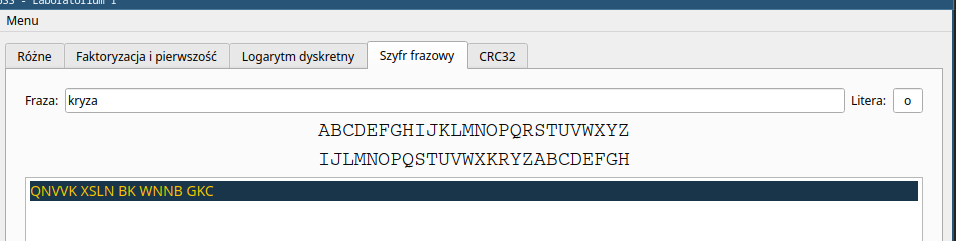
\includegraphics[width=1\textwidth]{eight.png} 
\paragraph{Odszyfrowałem ją: HELLO NICE TO MEET YOU \\}
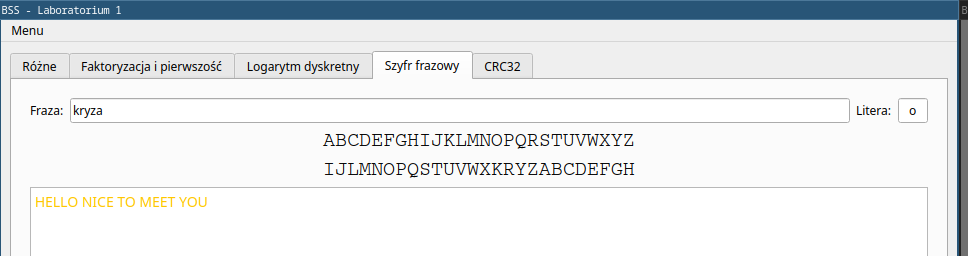
\includegraphics[width=1\textwidth]{nine.png}
\paragraph{Otrzymany klucz sesyjny zaszyfrowany: 423 65 693 1100 8 \_1073\_ \\ po odszyfrowaniu: 107, 114, 48, 122, 97, \_111\_ \\ po odkodowaniu: kryza, o }
\paragraph{Wiadomość zaszyfrowana: QNVVK XSLN BK WNNB GKC \\ Wiadomość odszyfrowana: HELLO NICE TO MEET YOU}
\section{Łamanie klucza prywatnego}
\paragraph{Z klucza publicznego otrzymałem $n_2 = 1763$}
\paragraph{Dokonałem faktoryzacji klucza publicznego $n = 43 \cdot 41$, p = 43, q = 41}
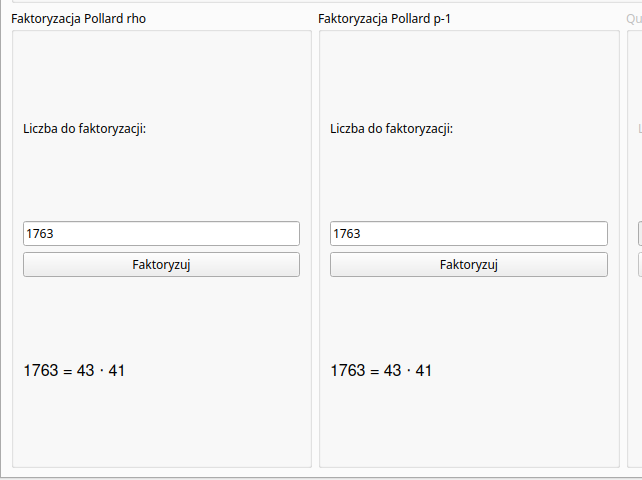
\includegraphics[width=1\textwidth]{ten.png}
\paragraph{Wyznaczyłem $\phi(n) = (p-1) \cdot (q-1) = 42 * 40 = 1680$}
\paragraph{Przygotowania do algorytmu Shanksa \\ c = 168, 1621, 1632, 665, 178 \_1734\_ \\  m = 68, 89, 90, 73, 79, \_67\_ \\  $n_2 = 1763$}
\paragraph{Algorythm Shanksa }
Algorytm z programu był dość zawodny, często nie dawał żadnych rezultatów, na przykład dla a = 168, y = 68, n = 1763 \\ 
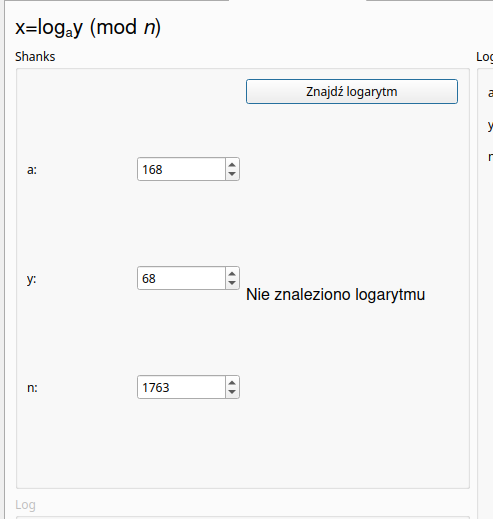
\includegraphics[width=1\textwidth]{eleven.png} \\ 
Algorytm zadziałał dla $a_1 = 1632, y_1 = 90, n = 1763$ dając wynik $d_s = 121$ \\ 
Algorytm zadziałał dla $a_2 = 665, y_2 = 73, n = 1763$ dając wynik $d_s = 23$ \\ 
Algorytm zadziałał dla $a_3 = 178, y_3 = 79, n = 1763$ dając wynik $d_s = 35$ \\ 
Algorytm zadziałał dla $a_4 = 1734, y_4 = 67, n = 1763$ dając wynik $d_s = 275$ \\ 
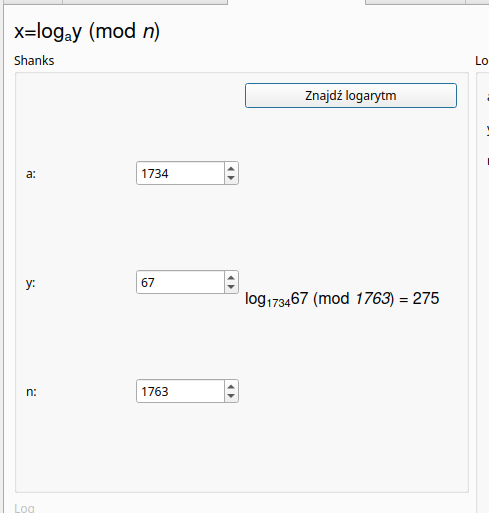
\includegraphics[width=1\textwidth]{twelve.png} \\ 
\paragraph{Sprawdziłem czy otrzymane wartości $d_s$ spełniają wymaganie $e \cdot d_s (mod \phi(n))$ \\}
\[ e = 11, d_s = \{ 121, 23, 35, 275 \}, n = 1763, \phi(n) = 1680 \]
\[ 11 \cdot \mathbf{121} (mod 1680) = 1331 \] 
\[ 11 \cdot \mathbf{23} (mod 1680) = 253 \] 
\[ 11 \cdot \mathbf{35} (mod 1680) = 385 \] 
\[ 11 \cdot \mathbf{275} (mod 1680) = 1345  \] 
Żadna z tych wartości nie spełnia wymagań
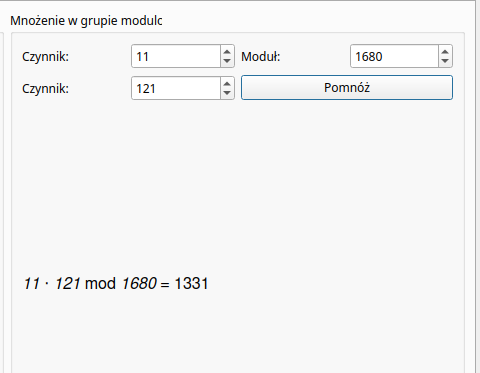
\includegraphics[width=1\textwidth]{thirteen.png} 
\paragraph{Następnie posłużyłem się metodą brutalną dla wartości które zadziałały przy Algorytmie Shanksa \\ }
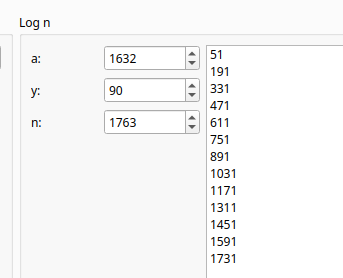
\includegraphics[width=1\textwidth]{fourteen.png} 
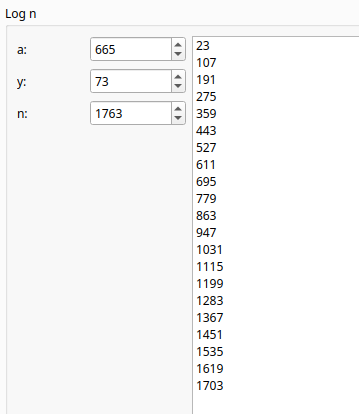
\includegraphics[width=1\textwidth]{fifteen.png} 
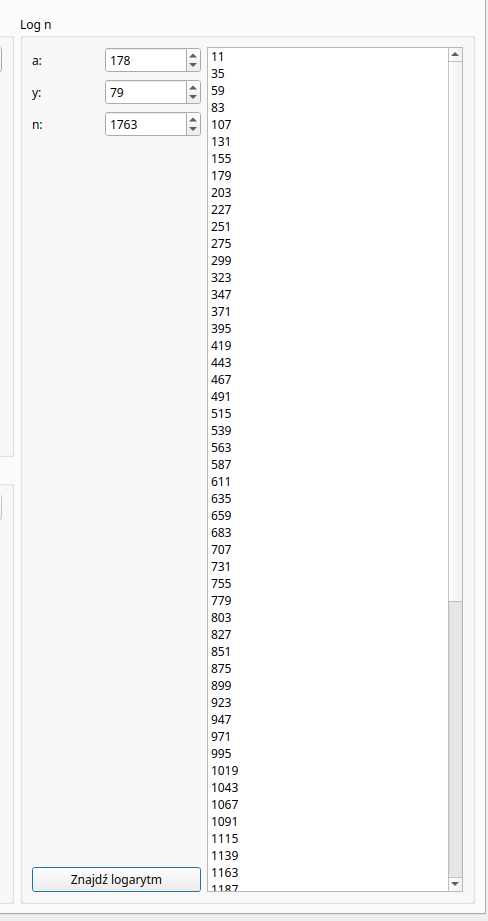
\includegraphics[width=1\textwidth]{sixteen.png} 
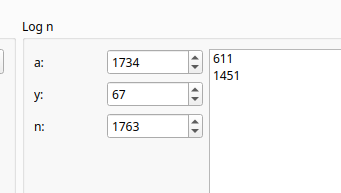
\includegraphics[width=1\textwidth]{seventeen.png} 
Dla e = 11, n = 1680, i d = 611 \\
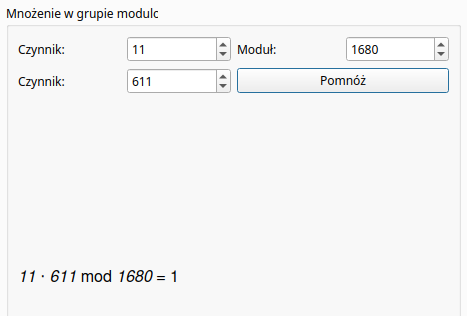
\includegraphics[width=1\textwidth]{eighteen.png} \\ 
d = 611 jest jednym z elementów klucza prywatnego, drugim jest $n_2 = 1763$
\section{Podpis Cyfrowy CRC}
\paragraph{Dla tekstu: PTAKI LATAJA KLUCZEM, wyznaczyłem wartość CRC: 2457674121 \\}
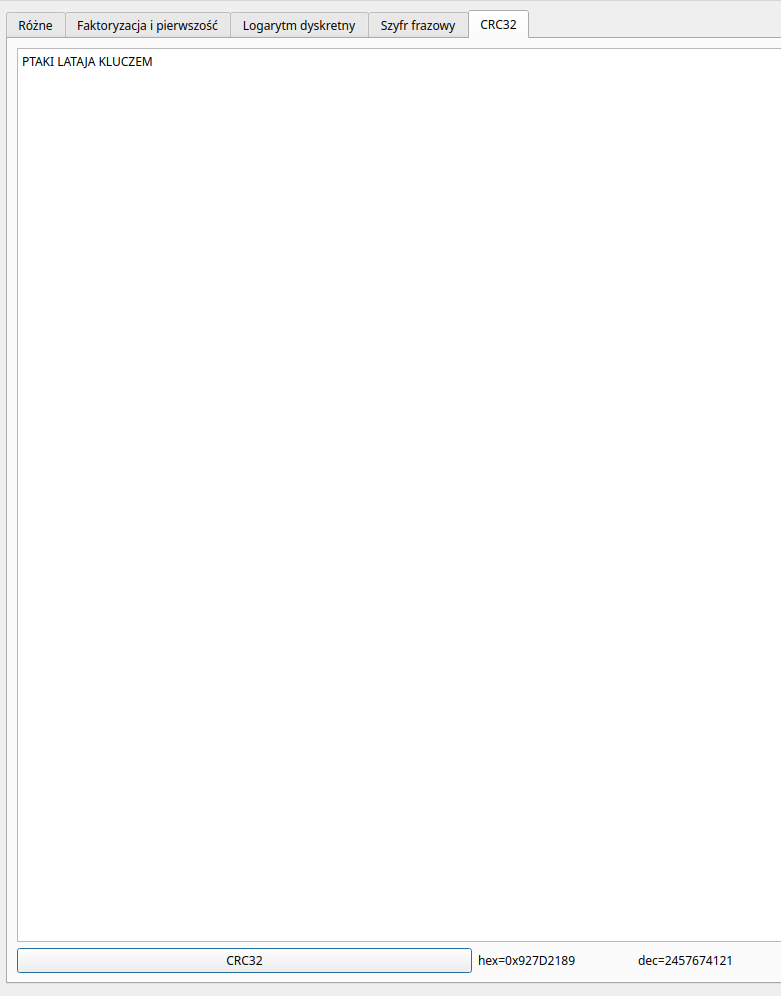
\includegraphics[width=1\textwidth]{nineteen.png} 
\paragraph{Podzieliłem na mniejsze grupy: 24, 57, 67, 41, 21}
\paragraph{Zaszyfrowałem wartość crc \\ d = 149, n = 1147 \\ Podpis cyfrowy: 890, 1091, 583, 617, 189 \\}
\paragraph{Wiadomość: PTAKI LATAJA KLUCZEM \\ Obliczona wartość CRC: 2457674121 \\ Klucz prywatny: d = 149, n = 1147, \\ Podpis cyfrowy: 890, 1091, 583, 617, 189}
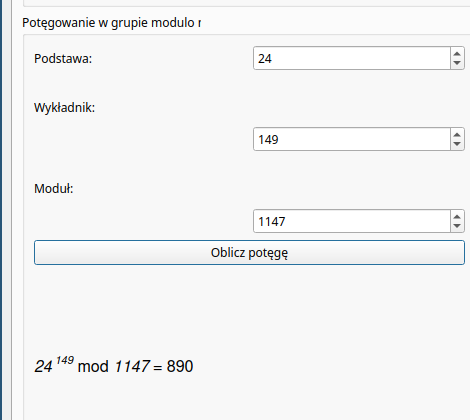
\includegraphics[width=1\textwidth]{twenty.png} 
\end{document}